% CHULOOPA Paper for AIMC 2026 - CONDENSED VERSION (4 pages max)
% Personal Drum Machines: User-Trainable Beatbox Classification with Real-Time AI Variations

\documentclass{aimc2026}

\usepackage[utf8]{inputenc}
\usepackage[T1]{fontenc}
\usepackage{hyperref}
\hypersetup{
  colorlinks = true,
  urlcolor   = blue,
  linkcolor  = black,
  citecolor  = black
}
\usepackage{url}
\usepackage{booktabs}
\usepackage{amsfonts}
\usepackage{nicefrac}
\usepackage{microtype}
\usepackage{graphicx}
\usepackage{grffile}
\usepackage[table]{xcolor}
\usepackage{colortbl}
\usepackage{amsmath}
\usepackage{cleveref}
\usepackage{dblfloatfix}

\hyphenation{beat-box beat-box-ing ChucK CHULO-OPA}

\title{Loops That Listen: A Voice-Controlled Dynamic Drum Looper with AI Variation}

\author{Anonymous Authors}

\begin{document}

\twocolumn[%
  \maketitle
  \begin{abstract}
    Live looping constrains musical dynamics. The same pattern cycles indefinitely, while a performance demands response and variation. CHULOOPA is a real-time drum looper that resolves this tension directly. The performer beatboxes patterns, and the system varies them in response to the live musical energy. A dBFS-mapped RMS measure, ``spice'', drives selection from a pre-generated bank of five variations. These variants are generated at different temperatures in parallel by a grid-based decoder-only transformer and then sorted by deviation score to maintain a predictable creativity spectrum for the performer. At each loop boundary, the variant matching the current spice level is selected without interrupting playback. CHULOOPA demonstrates that the loop's inherent repetition need not be a creative constraint. With audio-responsive AI variation, a loop becomes dynamically expressive without displacing the performer's musical intent.
  \end{abstract}

  \textbf{Keywords:} dynamic looping, audio-driven variation, spice detection, grid-quantized variation, co-creative AI, live performance
]

\thispagestyle{firstpage}

\section{INTRODUCTION}

The strength of a loop is also its main constraint: once recorded, it never changes. For drum loops in live performance, this constraint is especially pronounced. Where a live drummer would subtly add fills, vary dynamics, or shift the groove to match the moment, a drum loop plays back identically every cycle. While not always undesired, with hardware loop pedals like the BOSS RC-1 and software tools such as Ableton Live's Session View excelling at stacking static loops to provide rhythmic stability to a performance, an unchanging loop lacks the organic variation that makes live drumming compelling. With that limitation in mind, how can dynamic musicality be brought into drum loops without sacrificing their stability?

CHULOOPA (ChucK-based \citep{wang2015chuck} Loop Operator for Performance Audio) is a voice-controlled dynamic drum looper that addresses this. Unlike prior intelligent loopers~\citep{marchini2017reflexive,burloiu2020rolypoly} that work from guitar audio or pre-loaded MIDI drum scores, CHULOOPA uses voice input as its sole creation interface: a performer beatboxes a drum pattern, the system transcribes it in real-time via a user-trained KNN classifier, loops it, and immediately generates a bank of 5 AI variations at different creative levels. Simultaneously, the variant controller reads the live audio energy, \emph{spice}, and at each loop boundary performs a weighted probabilistic selection from the variation bank to match the current musical moment, without manual intervention.

\begin{figure*}
  \centering
  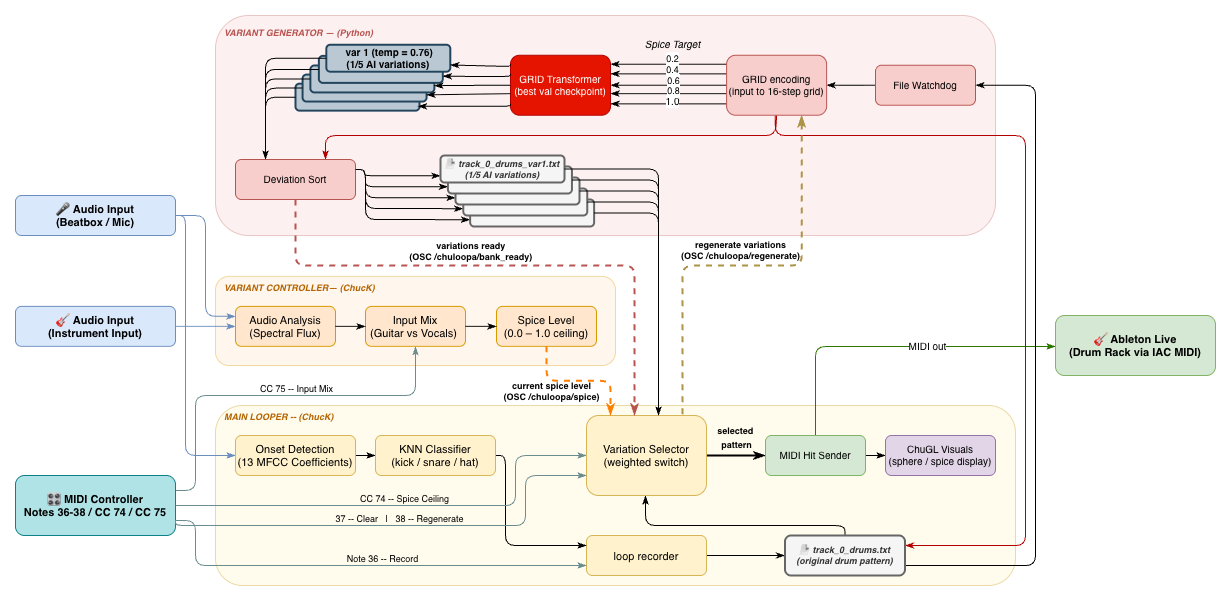
\includegraphics[width=\textwidth]{images/chuloopa_condensed_AIMC.png}
  \caption{\textbf{CHULOOPA system architecture}. Three concurrent processes communicate via OSC: main looper, variant generator, and variant controller.}
  \label{fig:system_diagram}
\end{figure*}

\section{RELATED WORK}

CHULOOPA builds on three prior bodies of work: intelligent loopers, generative models for drum pattern variation, and personalized beatbox classifiers for real-time percussion transcription.

\textbf{Intelligent Loopers.} From Pachet's Continuator \citep{pachet2003continuator} and OMax \citep{assayag2006omax}, which pioneered real-time style learning and pattern recombination from live input, to the Reflexive Looper \citep{marchini2017reflexive}, which established looping agents that adapt to a musician using constrained optimization to schedule material across upcoming beats, intelligent loopers have pursued the same goal: making loops responsive to a live performer. Rolypoly\textasciitilde{} \citep{burloiu2020rolypoly} takes a complementary approach, using RNNs pretrained on drum groove data to adapt the microtiming and velocity of a loaded drum score to a musician's timing, modulating how a pattern is played. The Living Looper \citep{shepardson2023living,shepardson2025evolving} extends this lineage: rather than replaying recorded audio, each loop channel uses a pre-trained RAVE autoencoder to project the recording into a latent space, where a lightweight linear model is fit per-recording, allowing the loop to drift and transform over time. \citet{madaghiele2025maal} push this toward full autonomy: their Multi-Agent Autonomous Looper (MAAL) assigns a rule-based agent to each loop track; agents continuously evaluate the rhythmic and harmonic compatibility of incoming live segments and autonomously decide what to loop, removing manual record triggers entirely. \emph{Recursive Speculation}~\citep{madaghiele2025recursive} demonstrates this with vocal input, where MAAL autonomously samples and layers a performer's improvised extended techniques into evolving looped structures.

\textbf{AI Drum Variation.} \citet{nuttall2021transformer} first trained a Transformer-XL on the Groove MIDI Dataset (GMD) for drum sequence generation; \citet{haki2022realtime} subsequently demonstrated real-time Transformer-based drum accompaniment in performance contexts. \citet{evans2024groovetransformer} extended this line of work into the GrooveTransformer, a VAE-based Eurorack module for real-time generative drum sequencing. GrooveTransformer steers variation through two pre-selected latent anchors and live MIDI input; it does not derive selection from raw audio energy, and generation is bounded by those reference points rather than a single live-recorded loop. \citet{bruford2020jaki} present jaki, which generates 1-bar LSTM continuations of a seed drum pattern and tunes them to user-defined musical features (syncopation, density, repetition) via deep reinforcement learning. \citet{alain2020deepdrummer} use active learning to converge on user drum-loop preferences from like/dislike ratings. \citet{brosnan2026darc} present DARC, a drum accompaniment model that conditions on musical context and a rhythm prompt (e.g.\ beatboxing), targeting music prototyping rather than live performance.

\textbf{Beatbox Transcription.} Mapping vocal percussion to drum classes is a cross-modal transcription task: \citet{santos2025tapscription} formalize it as mapping arbitrary percussive inputs to kick/snare/hat labels. \citet{delgado2019dataset} showed that vocal percussion styles vary significantly across amateur performers, and \citet{ramires2018user} demonstrated that personalized, user-specific classifiers substantially outperform generic models because different users produce acoustically distinct vocal percussion for the same drum class. \citet{martanto2025beatbox} confirms that KNN with MFCC features achieves strong accuracy for voice-derived percussion. Under live performance latency constraints, \citet{stowell2010beatbox} demonstrated real-time beatbox classification using delayed decision-making, and \citet{weber2024realtime} showed that high-quality drum transcription is achievable with minimal training data. Together, this body of work prioritizes personalization and real-time latency over generalization.

These three areas collectively motivate CHULOOPA's design: a personalized beatbox classifier trained on the performer's own voice, a Transformer-based variation bank for generation, and live audio energy as the autonomous selection signal, replacing manual variation control with continuous, performance-driven adaptation.

\section{SYSTEM DESIGN}
\label{sec:system}

CHULOOPA runs as three concurrent processes, color-coded in \Cref{fig:system_diagram}: the main looper (yellow) handles beatbox recording, drum classification, loop playback, and variation selection; the variant generator (red) generates a bank of five AI variations in the background the moment a new pattern is recorded; and the variant controller (orange) continuously monitors the live audio environment, streaming a single \emph{spice} value every 500\,ms. Separating spice detection into its own process was a deliberate design choice. Both the main looper and variant controller process live audio, but for different purposes: drum onset classification in the former and dBFS energy measurement in the latter.

\subsection{Beatboxing Classifier}

To initialize CHULOOPA, the performer first teaches the system their own beatboxing vocabulary. Rather than relying on a generic drum-sound dataset, CHULOOPA asks the performer to record 10 examples each of kick, snare, and hi-hat, creating a small personalized classifier that adapts to the performer’s vocal timbre and articulation in under two minutes.

The system extracts 13 MFCC coefficients per onset, a standard count for short audio classification tasks~\citep{martanto2025beatbox}. A KNN classifier~\citep{cover1967nearest} ($k$=3), implemented via ChAI's \texttt{KNN2} object~\citep{li2024chai}, trains automatically at startup in under one second. KNN was chosen deliberately: it performs well with as few as 30 samples, trains instantly, and requires no hyperparameter tuning. User-specific training constrains the problem space enough that a simple classifier suffices.

\subsection{Real-Time Transcription}

Immediate audio feedback during recording is central to CHULOOPA's performance model: the performer hears classified drum samples in real-time while beatboxing, allowing technique correction before committing a pattern to loop. This requires reliable onset detection and sub-30\,ms classification latency.

\textbf{Onset Detection:} Spectral flux with adaptive thresholding (1.5$\times$ running mean) in 512-sample frames, 128-sample hop (75\% overlap). The 512-sample frame provides 86\,Hz frequency resolution at 44.1\,kHz, necessary to discriminate kick fundamentals ($\sim$60--100\,Hz) from mid-frequency snare energy.

\textbf{Classification \& Playback:} Each onset is classified (kick/snare/hat) via MFCC-13 KNN and the corresponding drum sample plays immediately. Simultaneously, a MIDI note-on is sent to Ableton Live via the macOS Inter-Application Communication (IAC) driver, routing hits to a Drum Rack and giving the performer full control over drum sound design independently of the classification engine. Total input-to-playback latency is $\sim$25\,ms. Each hit is stored with delta-time encoding, the interval to the next hit or to loop end for the final hit, enabling drift-free loop playback. For AI variation, this timestamped sequence is quantized to a 16-step grid and written back as the active playback loop; the quantized version is then passed to the GRID model, ensuring the original and all variations share the same temporal reference.

\subsection{Spice Detection}

To autonomously select from the variation bank, we define \emph{spice} as a normalized measure of live audio energy that controls the selection of generated variations. The variant controller continuously measures the energy of the live performer and maps it to a spice value from 0.0 to 1.0, allowing CHULOOPA to autonomously respond to changes in musical intensity. RMS energy was chosen as the primary signal because it captures the cumulative acoustic energy of the room, with no additional sensing required. This intensity naturally invites more adventurous drumming, making it a reliable proxy for when variation is musically appropriate. Quieter passages favor conservative patterns; building energy pulls the system toward more adventurous ones.

The detector averages the RMS energy over a 500\,ms window and converts to a dBFS scale:

\begin{equation}
\text{spice} = \text{clamp}\!\left(\frac{\text{dBFS} - F}{P - F},\; 0.0,\; 1.0\right)
\label{eq:spice}
\end{equation}

where $F$ is the noise-floor threshold (--75\,dBFS) and $P$ is the expected peak performance level (--50\,dBFS). The dBFS mapping was chosen deliberately: a linear RMS scale would compress most of the musically-useful dynamic range near zero, whereas loudness perception is logarithmic

In performance mode, with a two-channel audio interface, the input mix knob blends the instrument and vocal inputs before analysis, so spice reflects the collective energy of the full performance rather than the beatboxer's voice alone. The 500\,ms window smooths over transient spikes while remaining responsive to sustained shifts in musical energy. Spice is streamed to the main looper process via OSC every 500\,ms.

\subsection{AI Variation Bank}

\textbf{Variation model:} CHULOOPA's generation engine is a grid-based decoder-only transformer (GRID), a 6-layer model with 256-dim embeddings, 8 attention heads, feed-forward dimension 1024, 42-token vocabulary, and 4.8M parameters, trained on the Expanded Groove MIDI Dataset~\citep{callender2020improving}. Bar pairs are constructed from performances containing at least two bars; pairs with empty bars or adjacent duplicates are discarded, yielding 12,085 training pairs. The model is conditioned on bar \emph{pairs}: given a context bar, it generates the immediately following bar. A masked loss is applied only to the continuation bar, training the model to predict the next bar rather than reconstruct the context. Patterns are quantized to a 16-step grid and encoded as alternating P\{step\}/N\{pitch\} tokens; generation terminates at a learned end-of-sequence marker.

When a loop is recorded, the variant generator immediately launches five parallel generation threads, one per spice target (0.2, 0.4, 0.6, 0.8, 1.0), chosen to maximise coverage of the spice spectrum while keeping generation overhead tractable; finer granularity would produce negligible perceptual difference between adjacent variants. Following the same encoding process, each thread feeds the recorded pattern as a GRID token sequence to the model, generating a new bar conditioned on the input. Each thread is assigned a sampling temperature that increases with its spice target ($T = 0.6 + 0.8 \times \text{spice}$, giving $T\!=\!0.76$ for the lowest-target thread and $T\!=\!1.40$ for the highest), biasing each toward outputs of different adventurousness without guaranteeing it. A post-generation deviation sorting step enforces the final conservative-to-adventurous ordering.

Because temperature steers \emph{tendency}, not outcome, a high-temperature run may occasionally produce a more conservative variation. To ensure the spice axis is musically reliable, the five generated variants are sorted ascending by the tuple $(\max(0,\,\Delta_{\text{hits}}),\, V_{\text{new}})$, where $\Delta_{\text{hits}}$ is the signed hit count difference from the original and $V_{\text{new}}$ is the count of drum voice classes absent from the original~\citep{gillick2019learning}. Density increase is the primary criterion; new voice classes break ties within the same density bucket. Sparser variations are not penalised. After sorting, slot\,1 always holds the most conservative result and slot\,5 the most adventurous, independent of which thread generated it. The variant generator signals completion via OSC. Total generation time: 3--5 seconds on consumer CPU hardware, entirely offline. \Cref{fig:grid_pairs} illustrates this gradient: the original pattern shown alongside Var~1 (Low Spice), Var~3 (Medium Spice), and Var~5 (High Spice) as 16-step drum grids. Sparse additions at low spice give way to denser fills and new drum voices at high spice, confirming the sorted order.
\begin{figure}[t]
  \centering
  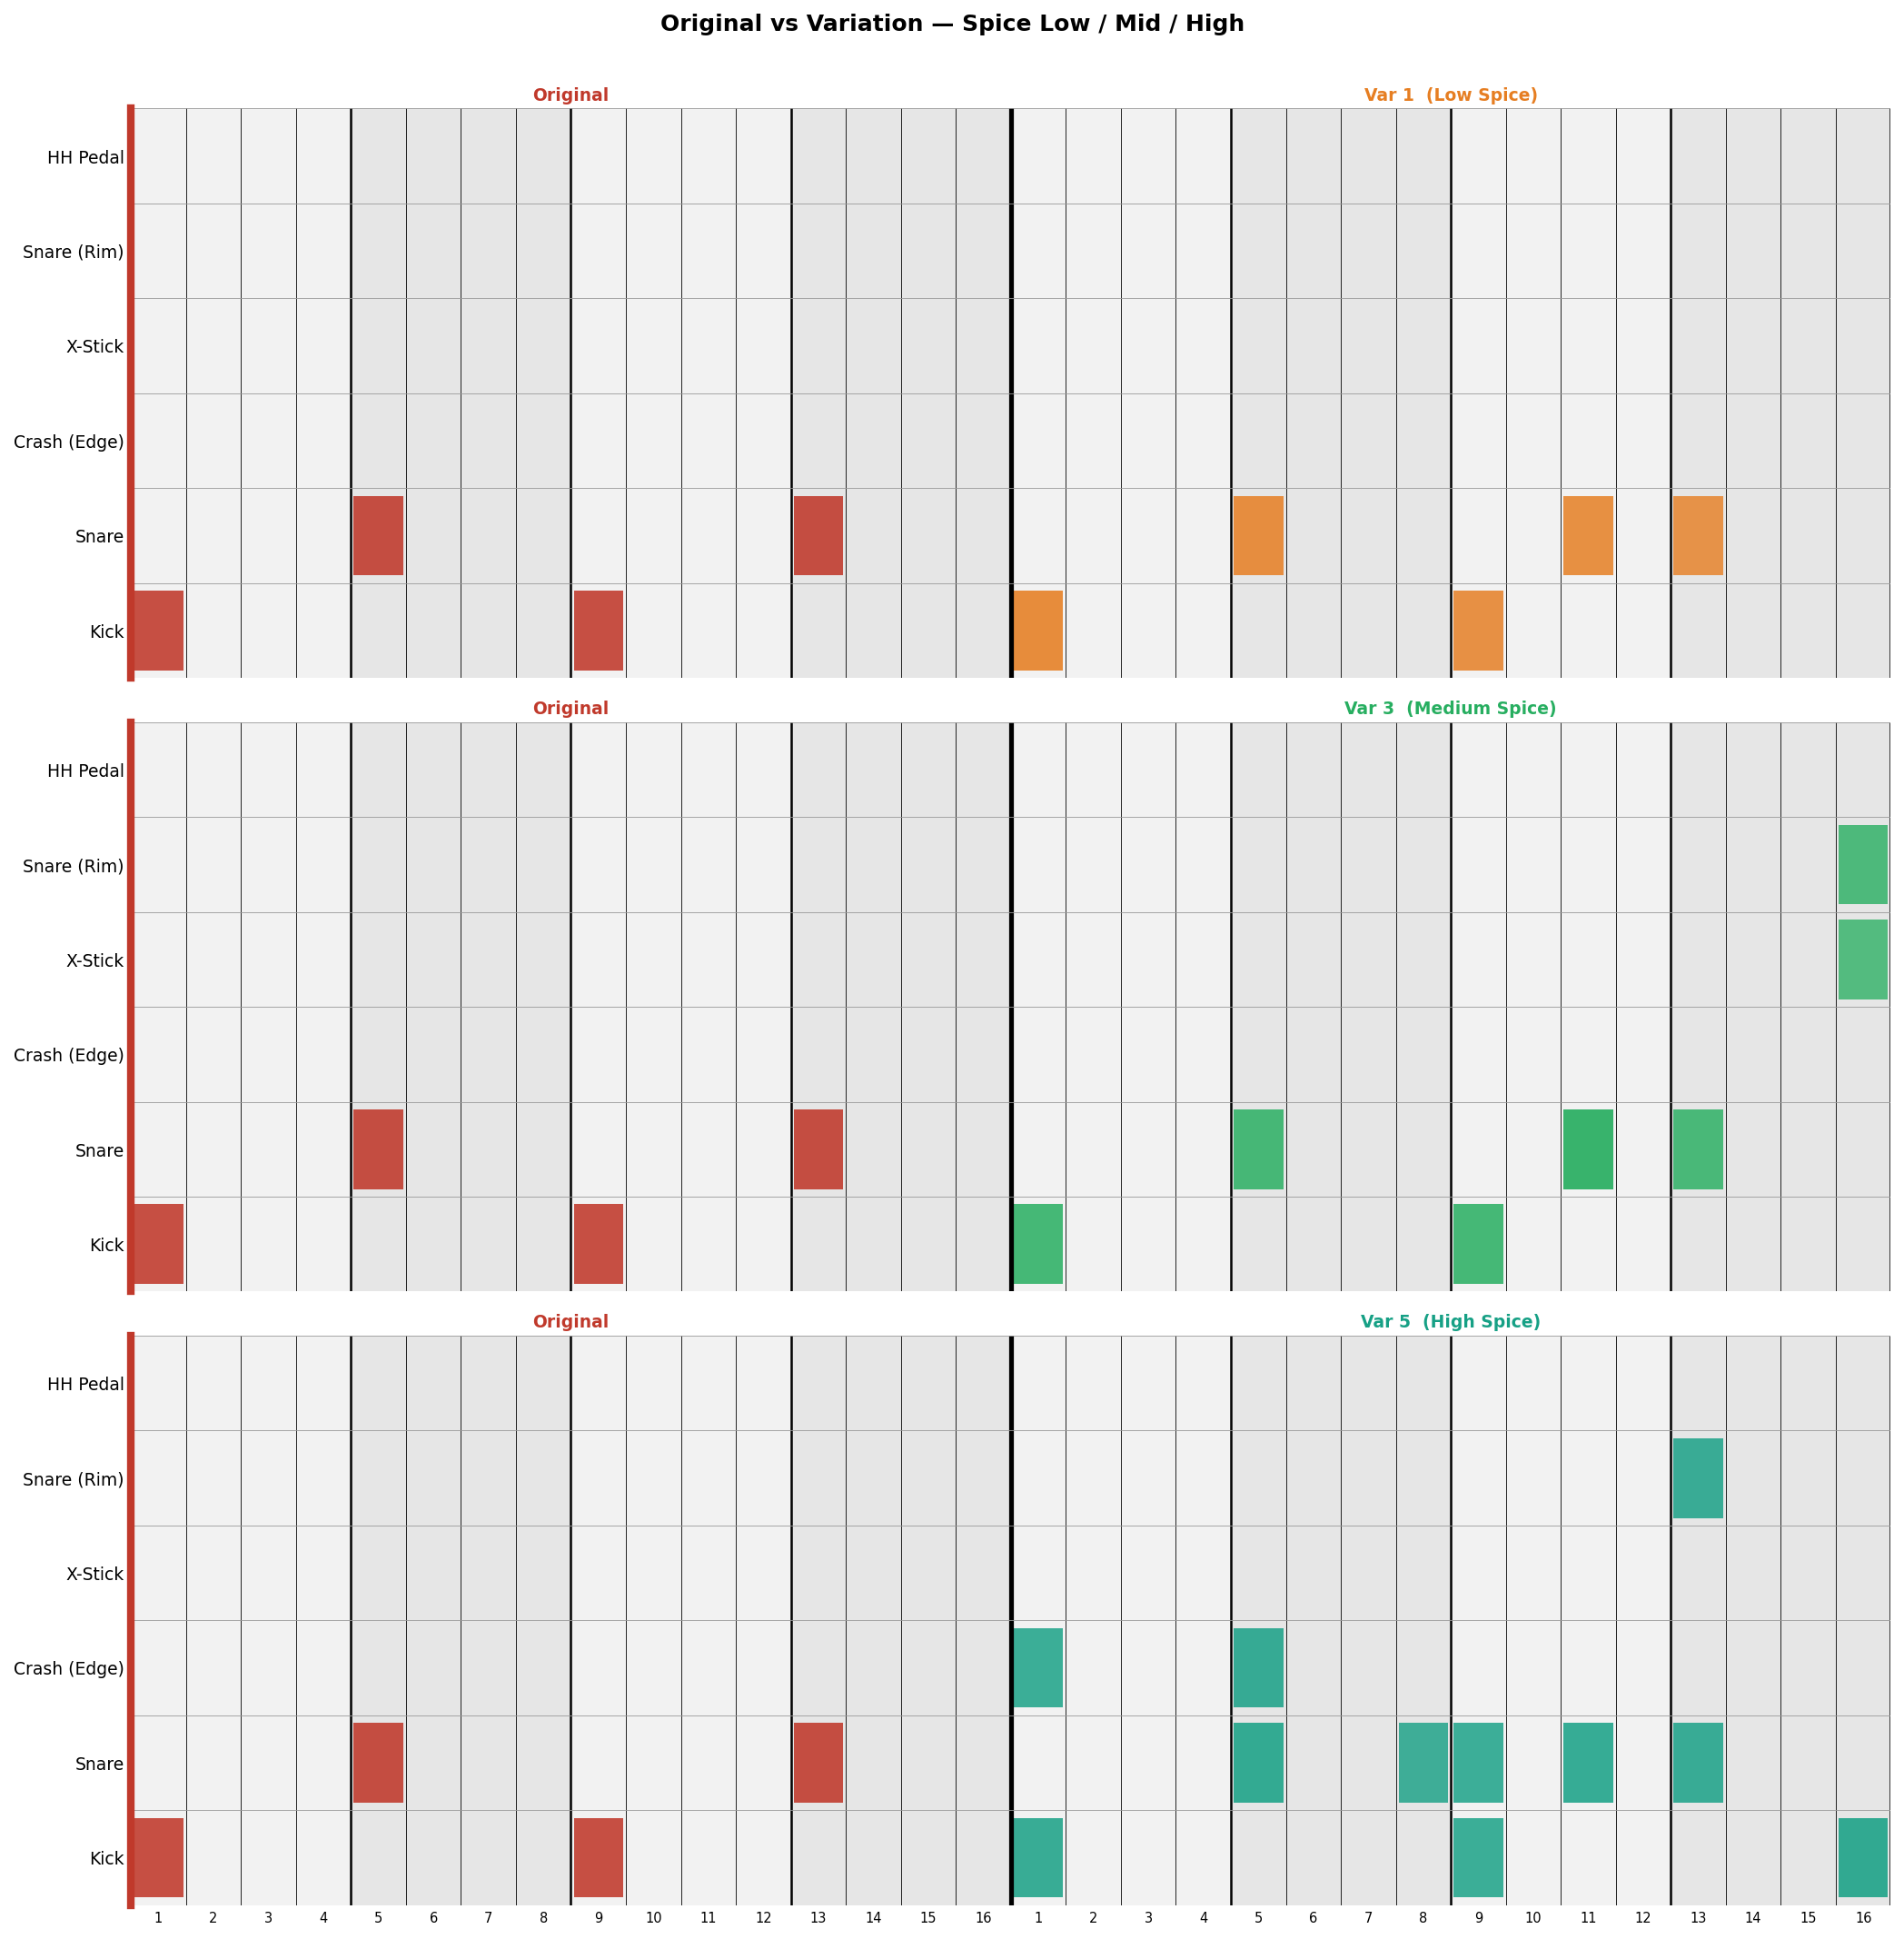
\includegraphics[width=\columnwidth]{images/grid_pairs_135.png}
  \caption{Drum grid comparison showing the original recorded pattern alongside AI-generated variations at low (Var~1), medium (Var~3), and high (Var~5) spice levels. Higher spice produces denser fills and introduces new drum voices (e.g.\ Crash (Edge) at high spice).}
  \label{fig:grid_pairs}
\end{figure}

\subsection{Weighted Variation Selection}

At each loop boundary, the main looper draws from a weighted distribution that shifts toward higher-numbered variants as spice rises (\Cref{tab:weights}). The distribution includes the original pattern as a valid option: at low spice the system may simply continue playing the original, treating restraint as a musical choice. Selection uses a \textbf{rolling 4-bar spice average}, with no variant playing more than twice consecutively.

\begin{table}[h]
\caption{Selection weights per spice tier. Cell shading indicates probability mass (darker = more likely). Values between tiers are linearly interpolated at loop boundaries.}
\label{tab:weights}
\centering
\small
\renewcommand{\arraystretch}{0.85}
\begin{tabular}{ccccccc}
\toprule
\textbf{Spice} & \textbf{Orig.} & \textbf{V1} & \textbf{V2} & \textbf{V3} & \textbf{V4} & \textbf{V5} \\
\midrule
0.00 & \cellcolor{red!60}0.50 & \cellcolor{red!48}0.40 & \cellcolor{red!12}0.10 & 0.00 & 0.00 & 0.00 \\
0.25 & \cellcolor{red!24}0.20 & \cellcolor{red!48}0.40 & \cellcolor{red!36}0.30 & \cellcolor{red!12}0.10 & 0.00 & 0.00 \\
0.50 & \cellcolor{red!6}0.05  & \cellcolor{red!24}0.20 & \cellcolor{red!48}0.40 & \cellcolor{red!36}0.30 & \cellcolor{red!6}0.05 & 0.00 \\
0.75 & 0.00 & \cellcolor{red!12}0.10 & \cellcolor{red!36}0.30 & \cellcolor{red!48}0.40 & \cellcolor{red!24}0.20 & 0.00 \\
1.00 & 0.00 & 0.00 & \cellcolor{red!24}0.20 & \cellcolor{red!48}0.40 & \cellcolor{red!36}0.30 & \cellcolor{red!12}0.10 \\
\bottomrule
\end{tabular}
\end{table}

The live performer retains creative control through a configurable spice \emph{ceiling}, mapped to \textbf{CC\,74}. Rather than selecting variations manually, the performer decides how much latitude to give the system to respond to the music accordingly.

\subsection{Live Performance Controls}

Inspired by hardware loopers, variation loading queues during the current cycle and executes at the next loop boundary, preventing mid-pattern interruptions. Each playback session holds a unique ID; scheduled drum hits validate their session before firing, eliminating overlap during transitions.

\textbf{MIDI Controls}: variation selection is fully automatic; no manual toggle required:
\begin{itemize}
  \item \textbf{Note\,36} (hold): record loop
  \item \textbf{Note\,37}: clear loop
  \item \textbf{Note\,38}: regenerate full variation bank
  \item \textbf{CC\,74}: spice ceiling (caps audio-driven selection)
  \item \textbf{CC\,75}: instrument/vocal input mix
\end{itemize}

\begin{figure}[t]
  \centering
  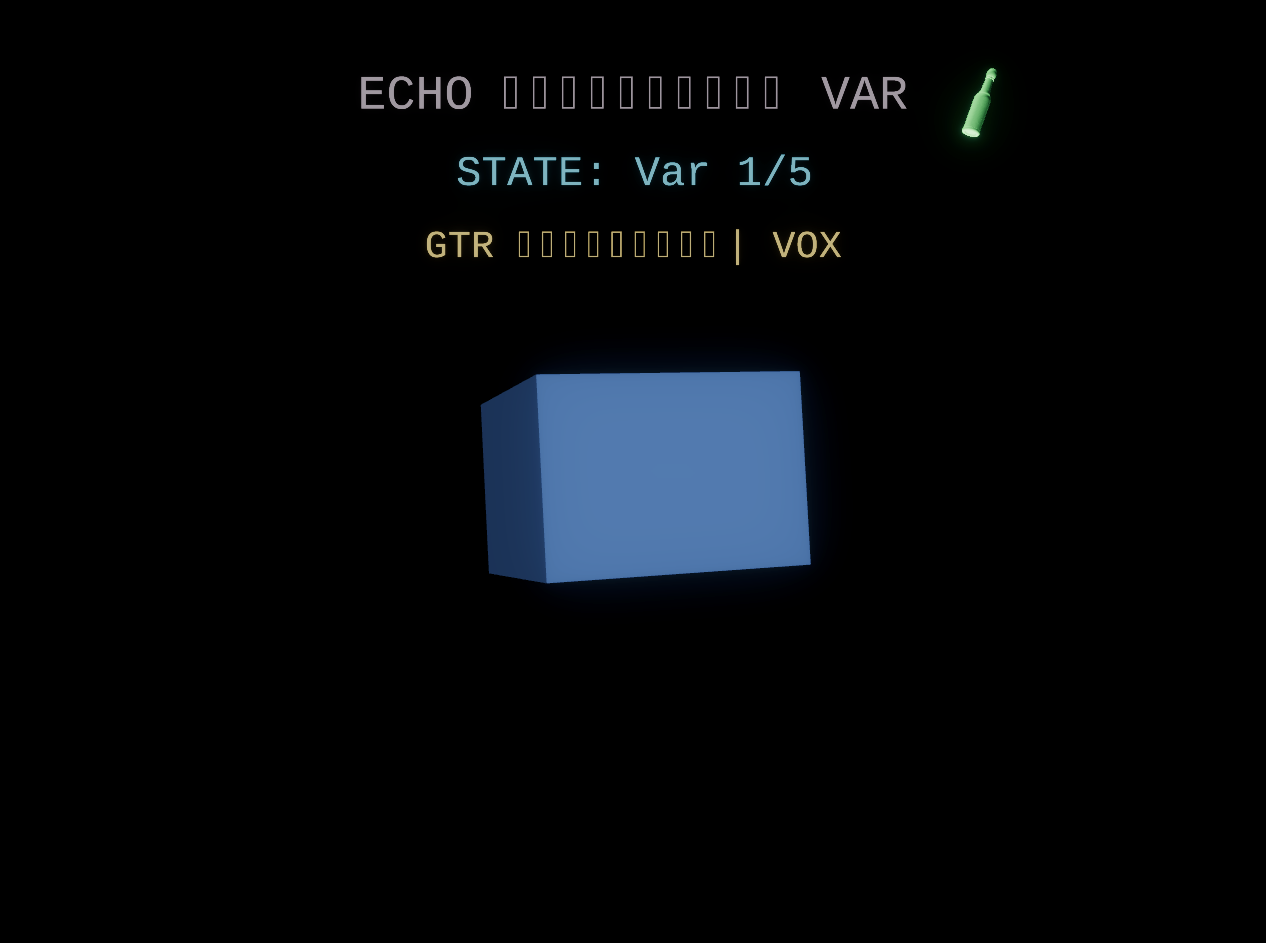
\includegraphics[width=0.8\columnwidth]{images/chuloopa_active_state_var1.png}\\[4pt]
  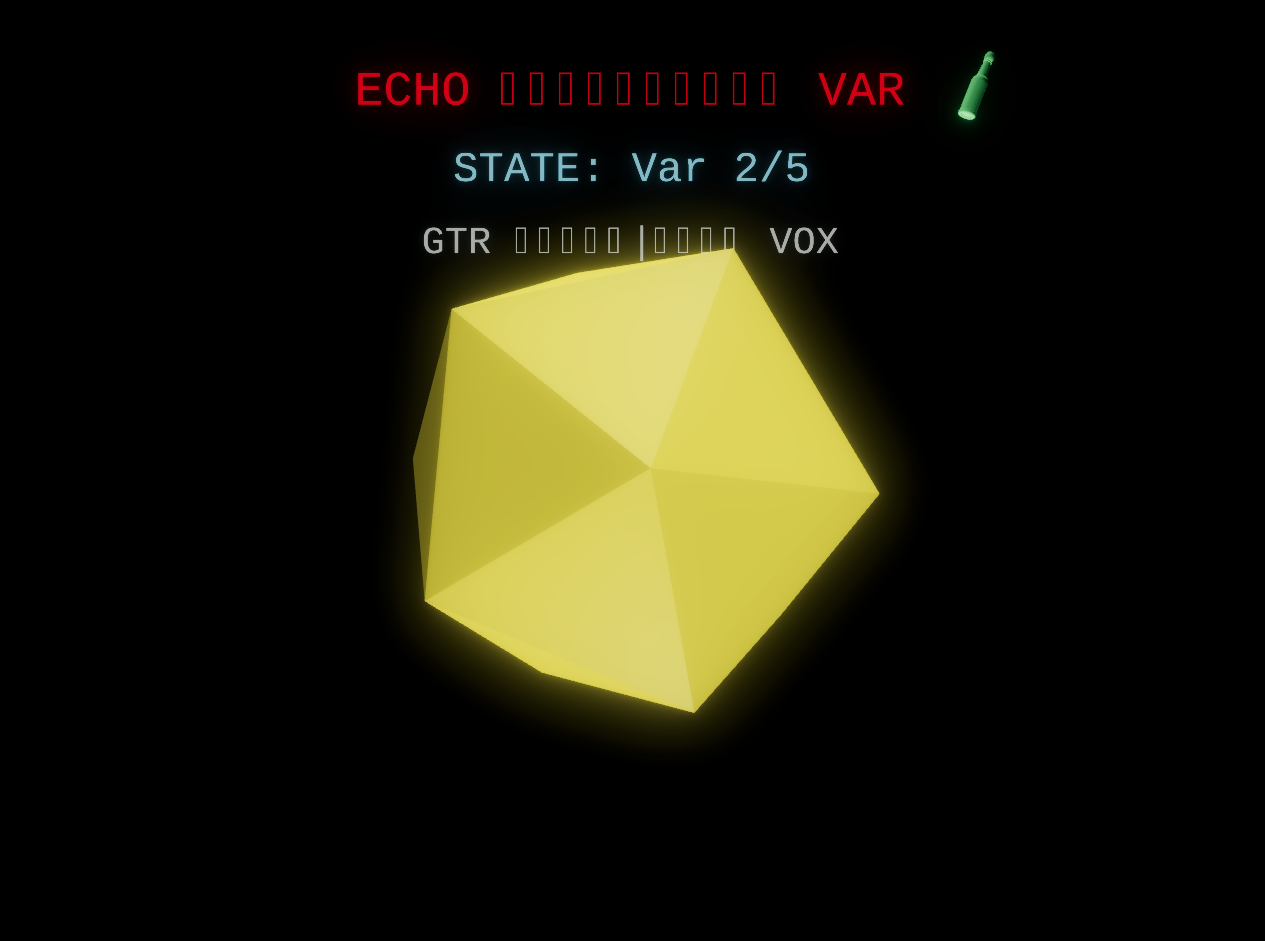
\includegraphics[width=0.8\columnwidth]{images/chuloopa_active_state.png}
  \caption{CHULOOPA performance UI. \textbf{Top:} Var\,1 at low spice (blue cube). \textbf{Bottom:} Var\,2 at high spice (yellow icosahedron). Color reflects the active variation slot (blue\,=\,Var\,1 through red\,=\,Var\,5); shape geometry tracks live spice independently (cube at low energy to icosahedron at peak).}
  \label{fig:active_ui}
\end{figure}

ChuGL~\citep{aday2024chugl} visual feedback (\Cref{fig:active_ui}) closes the loop for the performer: the central shape shifts color with the active variation slot (blue = Var\,1 through red = Var\,5) and pulses on each hit, while a spice slider reflects the instantaneous spice level. The color is discrete, updating at each loop boundary; shape geometry tracks live spice, shifting from a cube at low energy to an icosahedron at peak. A pulse fires at the moment each beatbox onset is classified, letting the performer confirm each hit in real time.


\section{EVALUATION}

The central evaluation question is whether CHULOOPA's AI-generated variations remain musically coherent with the human performance while offering a reliable, controllable range of complexity.

\subsection{Variation Coherence}

Variation coherence is evaluated by running 10 independent generation banks on a two-kick, two-snare pattern spanning 2.6 seconds. Each bank contains five variants at spice levels 0.2--1.0, deviation-sorted so slot\,1 is always the most conservative result and slot\,5 the most adventurous. Hit-probability heatmaps (\Cref{fig:heatmaps}) aggregate binary grids across all 10 runs; darker cells indicate more consistent activation.

\begin{figure}[t]
  \centering
  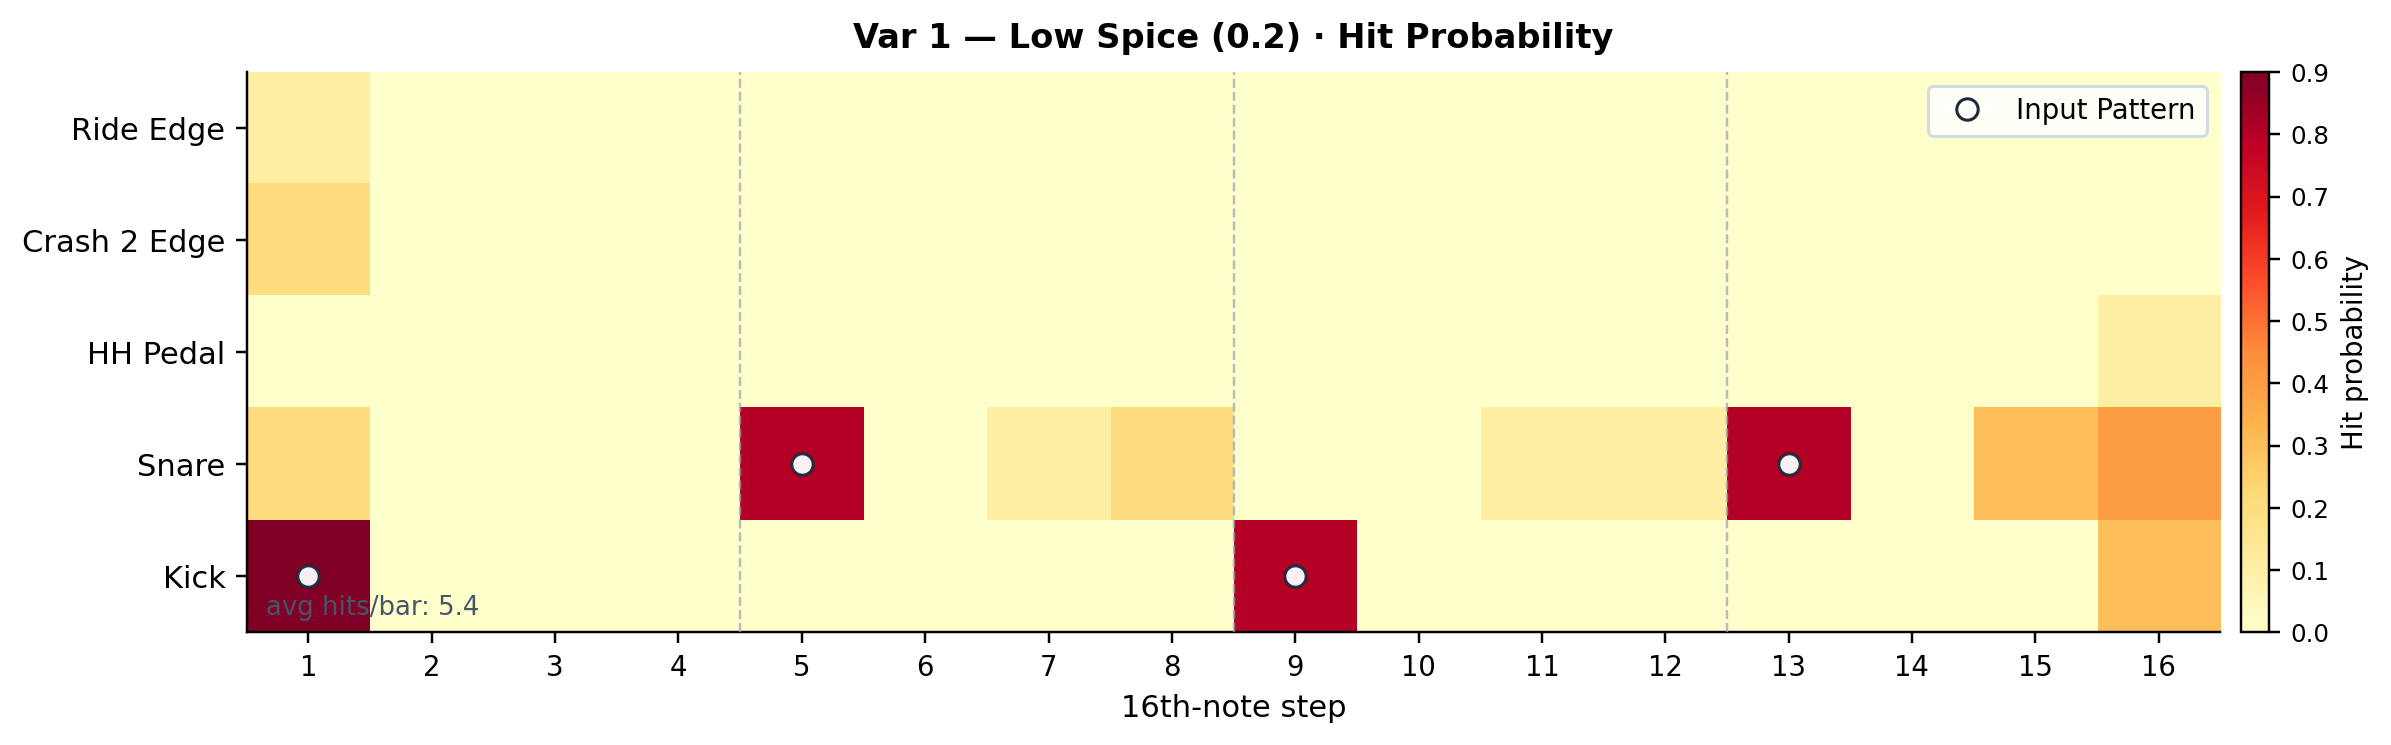
\includegraphics[width=\columnwidth]{images/eval_heatmap_test1_slot1.png}
  \vspace{2pt}
  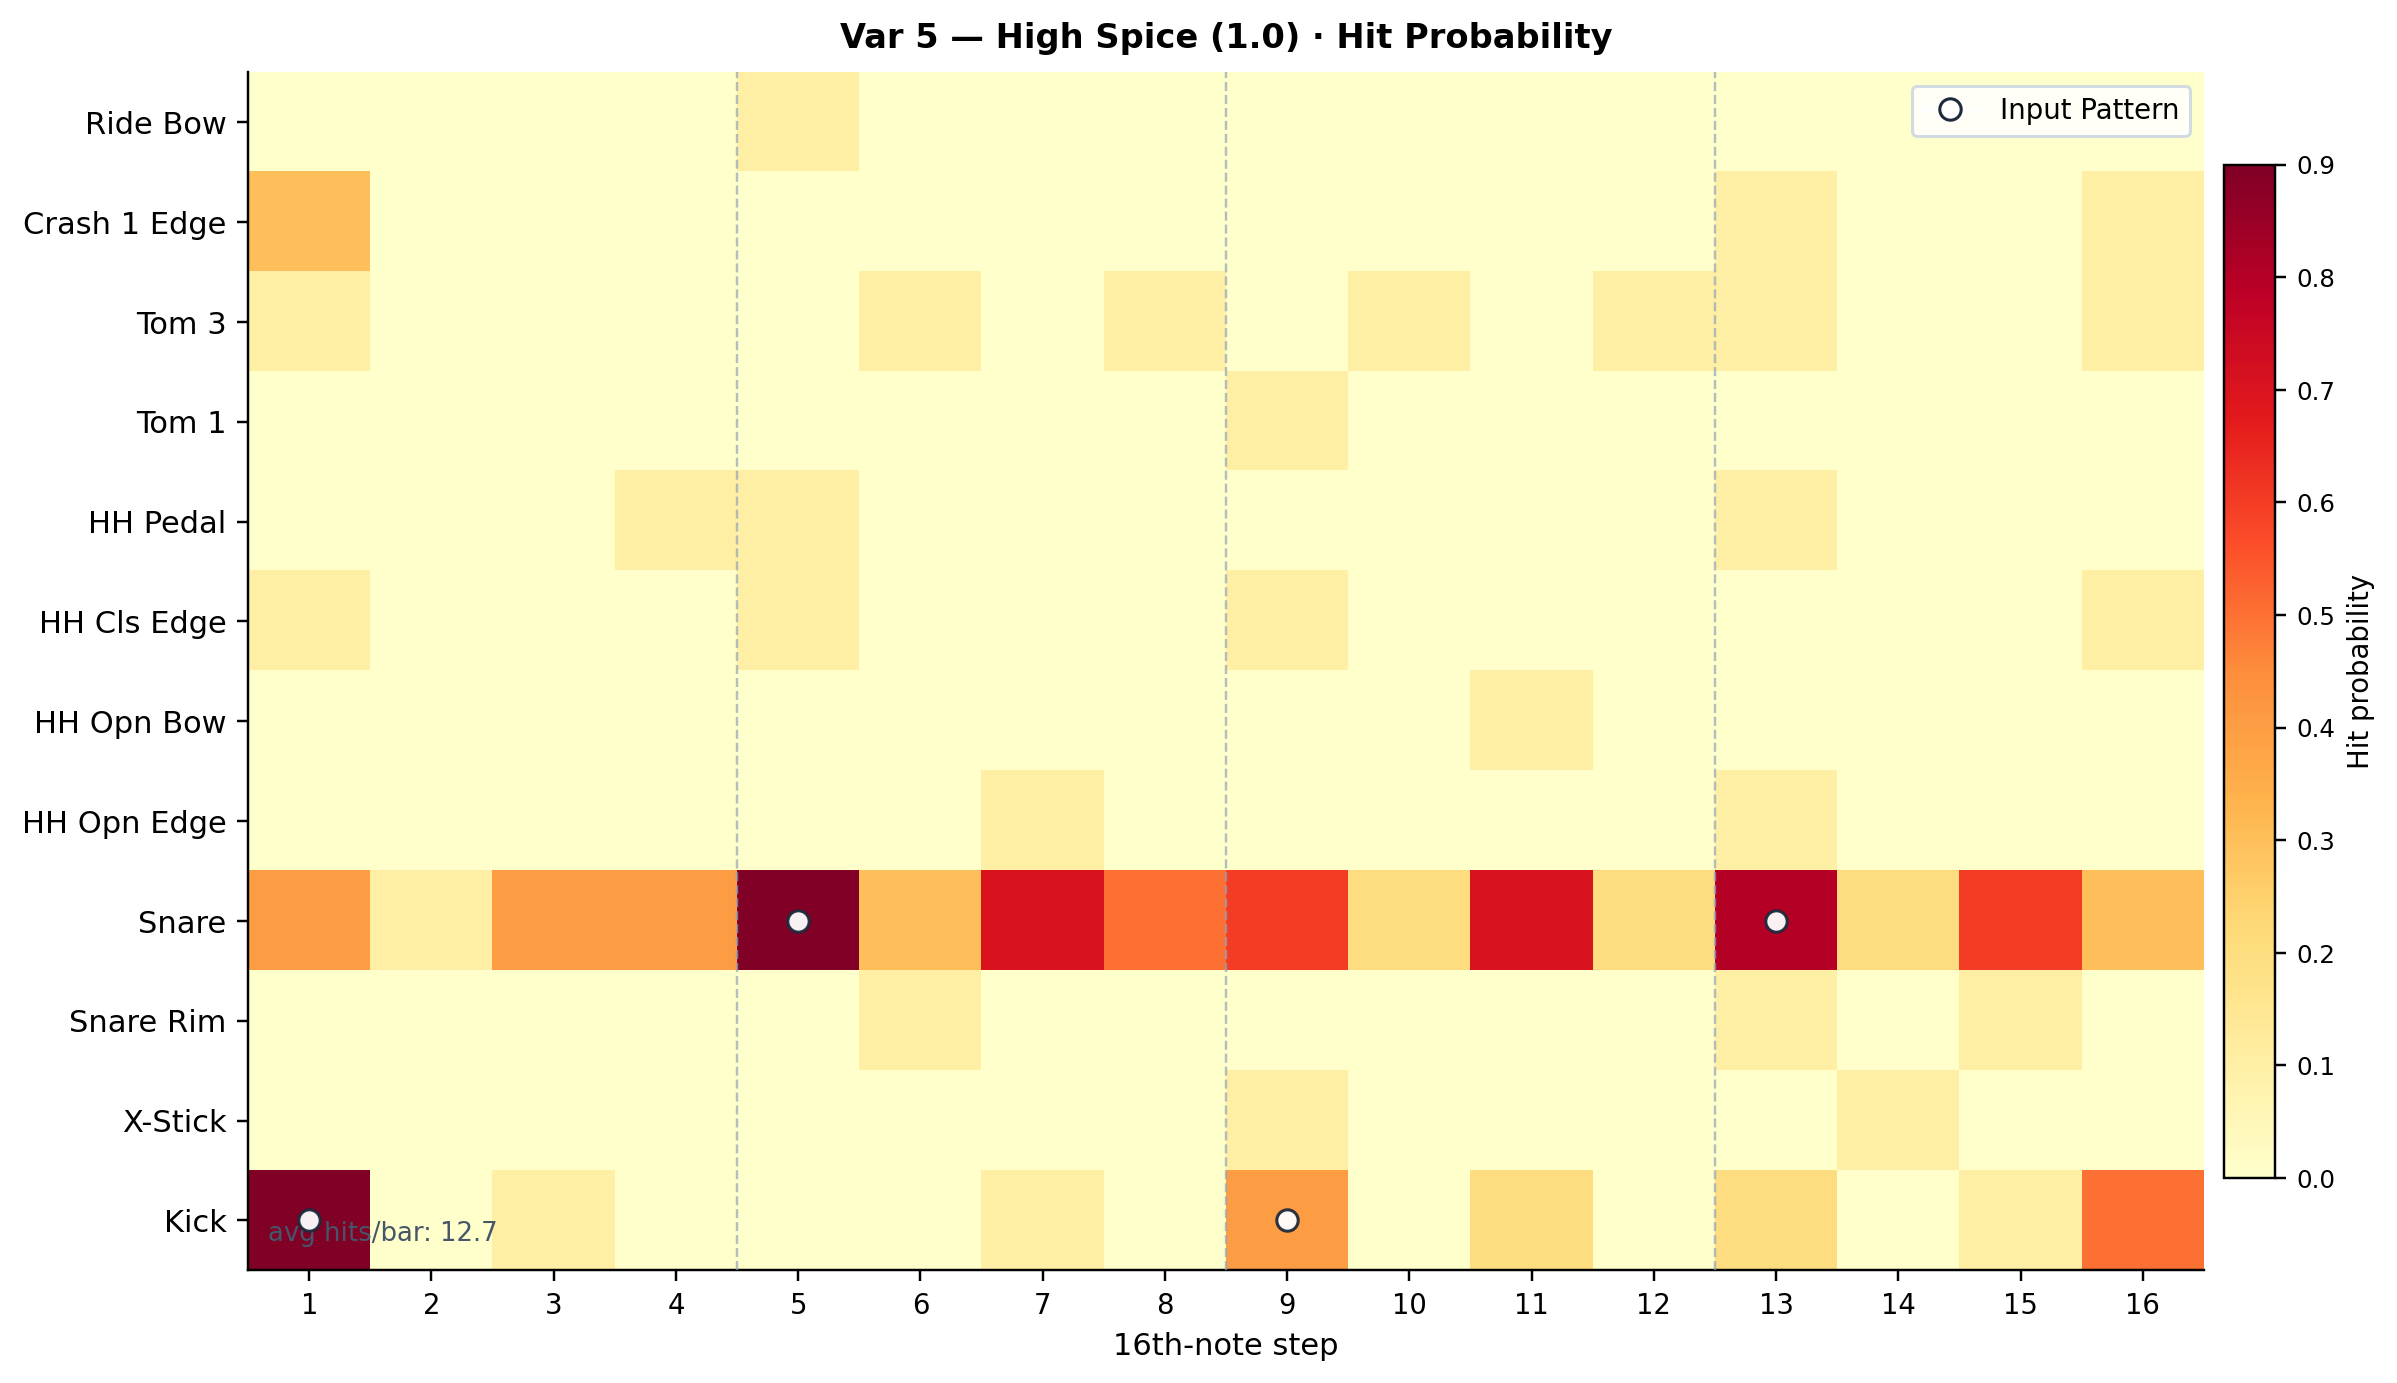
\includegraphics[width=\columnwidth]{images/eval_heatmap_test1_slot5.png}
  \caption{Hit-probability heatmaps for a simple kick--snare input, aggregated over $N{=}10$ independent banks. White circles mark input pattern positions. \textbf{Top:} Var~1 (Low Spice, 0.2): sparse additions, input positions dominant. \textbf{Bottom:} Var~5 (High Spice, 1.0): elaborated groove with hi-hats, toms, and snare fills; input anchors remain visible at step\,1 and step\,9.}
  \label{fig:heatmaps}
\end{figure}

At low spice, Var\,1 produces an average of 5.4\,hits/bar, with 82.5\% of input cells activating consistently, confirming strong input preservation. Additional voices appear at low probability (HH Pedal, Crash\,2 Edge, Ride Edge), representing occasional idiomatic ornamentation rather than structural additions. At high spice, Var\,5 reaches 12.7\,hits/bar: the snare row spreads broadly, the kick maintains its step-1 anchor, and hi-hat and tom voices emerge. Crucially, additions concentrate on a small fraction of non-input positions: averaged across all empty grid cells, activation probability remains below 4\% even at high spice (0.7\% at Var\,1, 3.1\% at Var\,5), confirming the model targets musically plausible positions rather than filling the grid at random. The density gradient (5.4~$\to$~12.7) confirms the spice axis produces a reliable complexity spectrum: the system generates sparser outputs at low spice and more elaborated ones at high spice, with input positions serving as structural anchors throughout.

\subsection{Aesthetic Observations}

The first author performed with CHULOOPA across multiple solo sessions, each lasting 10--20 minutes.\footnote{Demo and supplementary materials: \url{https://sites.google.com/view/chuloopa/home}} All generated variations were assessed as coherent musical ideas; the only failure cases could be traced to input-side quantization artifacts rather than output-side incoherence. The strict 16-step grid eliminates beat-drift entirely.

Mid-range spice values (approximately 0.4--0.6) proved most musically satisfying, neither too sparse nor too elaborate. Hearing the system return to the original pattern at low spice served as a rhythmic anchor, reinforcing awareness of the source groove. Unlike static loops, which can grow stale when brought to the forefront of the performance, CHULOOPA invites attention when given the spotlight. When holding a chord or leaving space in the arrangement, the variations shine as a musical statement in their own right, with the performer remaining compositionally in control.

\section{CONCLUSION}

CHULOOPA demonstrates that AI-generated variation can bring dynamic musicality to the drum loop without sacrificing its stability. At low spice, 82.5\% of original hit positions activate consistently across $N{=}10$ independent banks, confirming the model treats the performer's pattern as a structural anchor rather than a seed to discard. Deviation-sorted parallel generation produces a reliable density gradient, 5.4 to 12.7 hits/bar from slot~1 to slot~5, confirming the spice axis as a controllable complexity spectrum. Spice drives autonomous selection at each loop boundary, matching the variation to the current musical energy without demanding performer intervention. An AI looper can elaborate a groove without displacing it.

Current constraints are deliberate tradeoffs. The 16-step quantization grid is the source of CHULOOPA's temporal reliability, but it excludes swing feel, non-4/4 meters, and 32nd-note micro-timing. Variations are conditioned to continue from the input rather than replicate it, always coherent with the original but free to reinterpret it. Spice tracks amplitude alone, a reliable proxy for musical energy but blind to harmonic or rhythmic context. The evaluation is self-reported by the author; a structured listener study would strengthen the coherence claims.

Natural extensions include multi-track looping with coherent cross-track variation, swing and compound-meter support, and melodic generation. An open question is whether spice can be enriched by incorporating spectral complexity and rhythmic density alongside amplitude, and how drum patterns are expected to adapt to those changes, giving the selection engine a fuller picture of when variation is musically called for. The variation bank and autonomous selection together show that the loop's repetition can be its starting point, not its ceiling.

\section*{Author Declarations}

\textbf{Conflicts of Interest:} None.

\textbf{Ethical Issues:} No formal ethical review was required for this research. The GRID model was trained on the publicly available Expanded Groove MIDI Dataset (CC-BY 4.0).

\textbf{Use of AI:} Claude (Anthropic) assisted with technical implementation (system development, debugging) and paper writing (structuring, editing). All research design, conceptual decisions, and conclusions are the author's own. 

% \section*{Acknowledgments}
% Omitted for blind review.


\bibliographystyle{apalike}
\bibliography{references}

\end{document}
